\title{XOR Gate Digital Circuits}
\begin{document}
\section{XOR and XNOR Gates}

\begin{frame}{The XOR and XNOR operations}
  \begin{block}{Exclusive OR}
    We previous discussed the exclusive OR operation, which is spelled like this:
    $$X \oplus Y = X' \cdot Y + X \cdot Y'$$
    \begin{itemize}
      \item The XOR function produces a 1 if its inputs are different.
      \item Complementing any two signals (input or output) of a two input XOR gate does not change the result of the function.
    \end{itemize}
  \end{block}
  \begin{center}
    \begin{tabular}{cc|cc}
      X & Y & $X \oplus Y$ & $(X \oplus Y)'$ \\
      \hline
      0 & 0 & 0 & 1 \\
      0 & 1 & 1 & 0 \\
      1 & 0 & 1 & 0 \\
      1 & 1 & 0 & 1 \\
    \end{tabular}
  \end{center}
\end{frame}

\section{Parity}

\subsection{Parity Concepts}

\begin{frame}{Parity}
  \begin{definition}
    A sequence is said to have \alert{odd parity} if an odd number of bits are 1.  The sequence is said to have \alert{even parity} if an even number of bits are 1.
  \end{definition}
  Parity is general used for error detection in digital circuits.
  \begin{itemize}
    \item RAM
    \item RAID levels 3, 4, 5, and 6
    \item Communications devices
  \end{itemize}
  What are two limitations of parity error detection?
\end{frame}

\begin{frame}{Using XOR gates in a parity circuit}
  Using cascading XOR gates, we can create a parity checking circuit.\\
  \begin{center}
    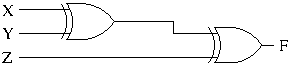
\includegraphics{CascadingParityCircuit}
  \end{center}
  Is this odd or even parity?  How would we use a similar circuit to check the other type of parity?
\end{frame}

\subsection{The 74x280 Parity Generator}

\begin{frame}{The 74x280 parity generator circuit}
  The 74x280 is a nine bit parity generator circuit.\\
  \begin{center}
    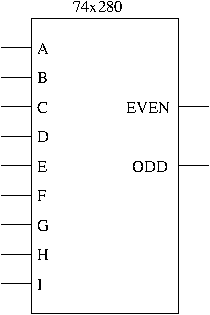
\includegraphics{74x280Schematic}
  \end{center}
  Why would this standard circuit use nine bits instead of something more normal, like eight?
\end{frame}

\begin{frame}{Parity detection in a memory circuit}
  \begin{center}
    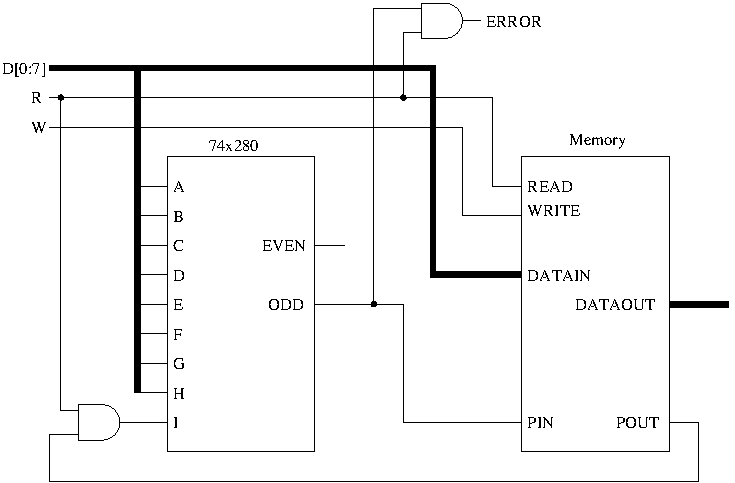
\includegraphics[scale=0.7]{MemoryCircuitParity}
  \end{center}
\end{frame}

Show the 74x280 parity circuit in VHDL.

\section{Comparators}
\subsection{Comparator Circuits Using XOR Logic}

\begin{frame}{Determining equality}
  \begin{definition}
    A \alert{comparator} circuit can be used to determine if two given sequences of bits are the same.  The XOR operation is a logical choice for this job.
  \end{definition}
  \begin{center}
    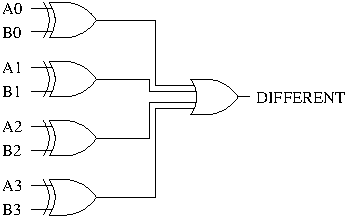
\includegraphics{ComparatorLogic}
  \end{center}
\end{frame}

\subsection{The 74x85 and 74x682 Circuits}

\begin{frame}{The 74x85 comparator circuit}
  This circuit compares two 4-bit inputs.\\
  \begin{center}
    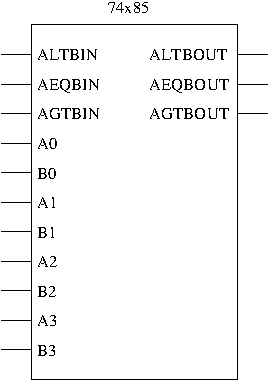
\includegraphics{74x85Schematic}
  \end{center}
\end{frame}

\begin{frame}{Cascading comparators}
  To compare more than four bits, we can cascade 74x85 chips.\\
  \begin{center}
    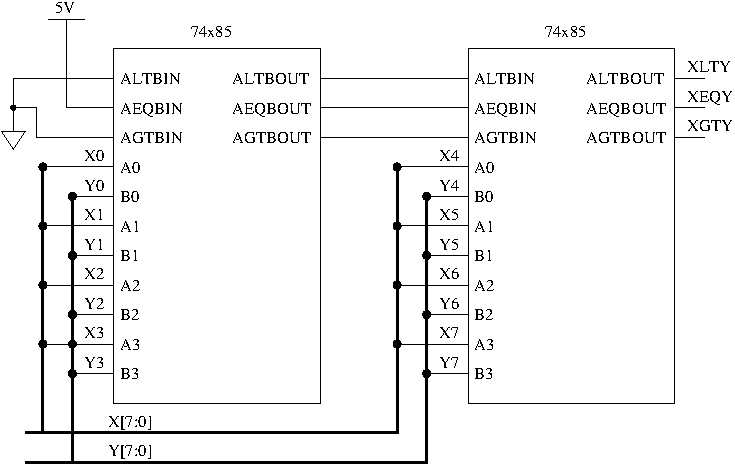
\includegraphics[scale=0.8]{EightBitComparator}
  \end{center}
\end{frame}

\begin{frame}{The 74x682 comparator circuit}
  The 74x682 provides an eight-bit comparator on in one chip.\\
  \begin{center}
    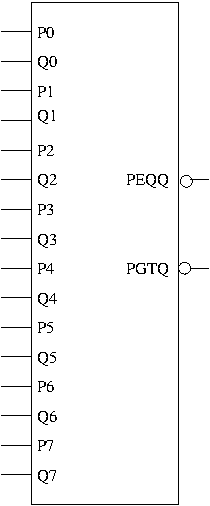
\includegraphics[scale=0.5]{74x682Schematic}
  \end{center}
  How can we find the standard algebraic comparions ($\neq, =, <, \leq, >, \geq$) based on the two outputs of the 74x682?
\end{frame}

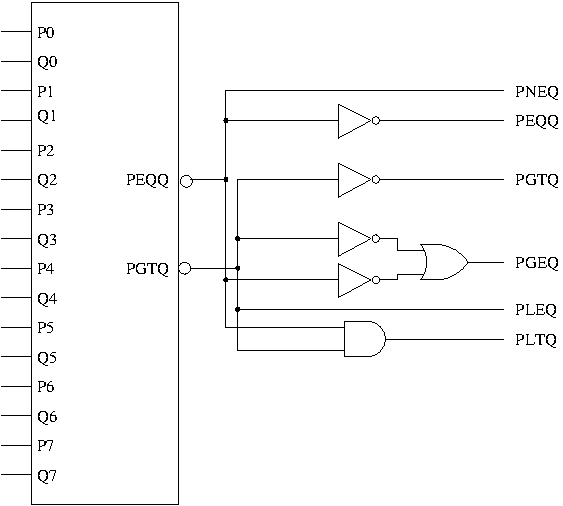
\includegraphics{74x682Extended}

\end{document}
